\section{Geometry}
\label{sec:geom}
This section describes the parameters and methods used to describe the
substructure geometry in \textit{FloatingSE}.  Note that at the time of this
writing, only generic spar and semisubmersible configurations are
currently implemented in the model.  Tension leg platforms (TLPs) and
other taut-mooring configurations will likely be added in the next
months.  These three classical substructure designs are shown in Figure
\ref{fig:archetype}.
\begin{figure}
  \begin{center}
    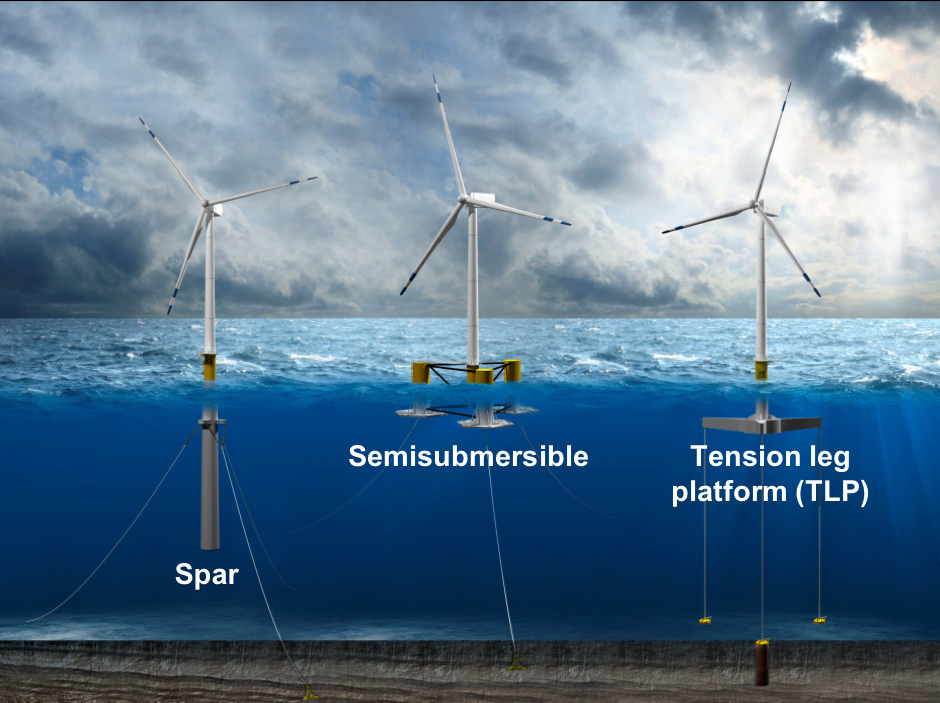
\includegraphics[width=3.75in]{figs/archetypes}
    \caption{Three classical designs for floating turbine substructures.}
    \label{fig:archetype}
  \end{center}
\end{figure}

The nomenclature used in \textit{FloatingSE} is borrowed from the field
of naval architecture.  The general configuration of a spar-type
substructure is shown in Figure \ref{fig:diagram}.  A semisubmersible
configuration would have multiple vertical columns connected with
truss and pontoon elements, but the parameterization of the overall
geometry is the same.
\begin{figure}
  \begin{center}
    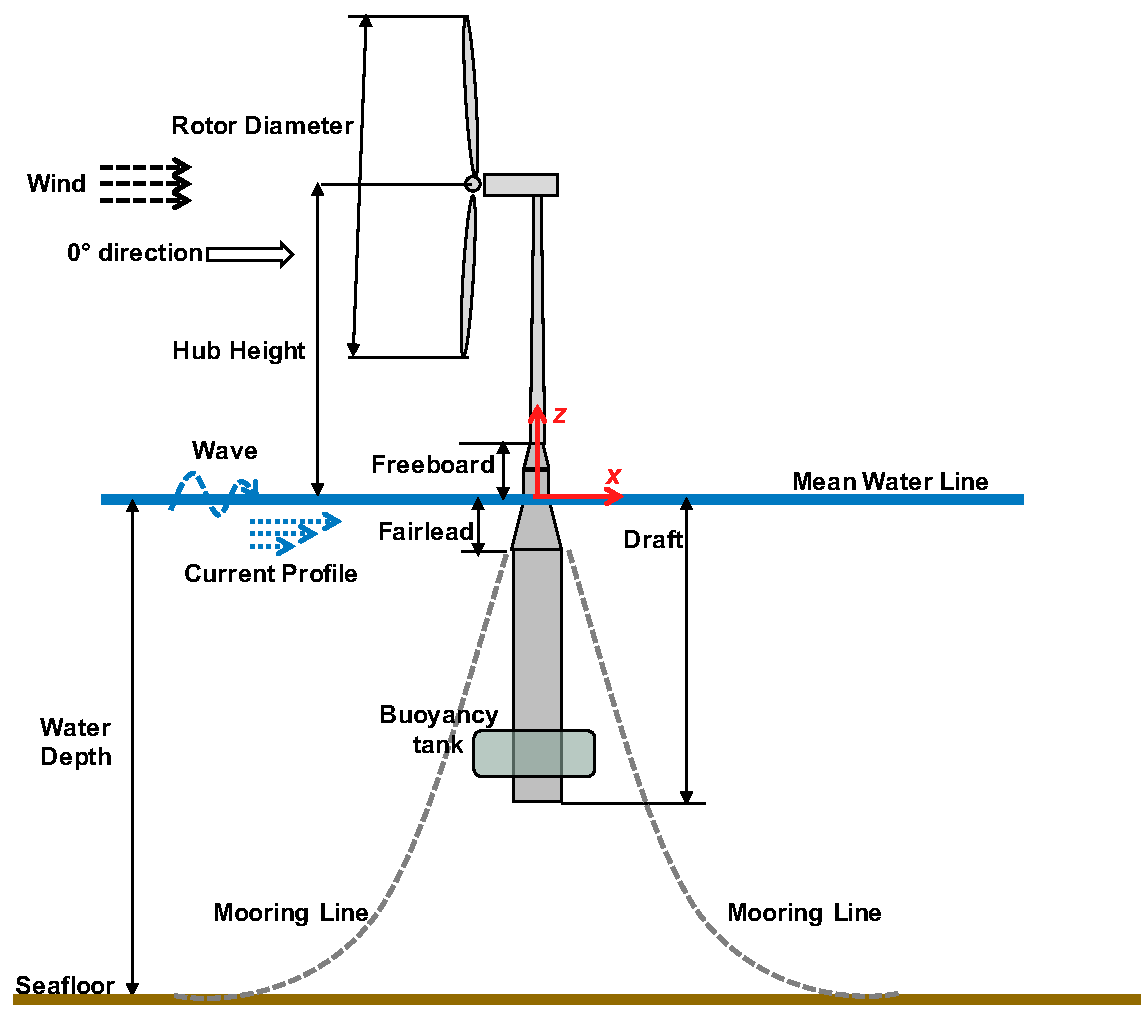
\includegraphics[width=5in]{figs/diagram}
    \caption{Geometry parameterization with common wind turbine and
      naval architecture conventions.}
    \label{fig:diagram}
  \end{center}
\end{figure}

\subsection{Discretization}
To allow for varying geometry parameters along the length of
substructure columns, the larger components are divided into sections.
The user may specify the number of overall sections and the geometry of
each section.  Some of the geometry parameters are tied to the nodes
that bound each section, such as column diameter and wall thickness,
with linear variation between each node.  Other parameters are
considered constant within each section, such as the spacing between
ring stiffeners.  The number of sections should resemble the physical
number of cans or sections used in the manufacturing of the real
article.  The examples provided in \textit{FloatingSE} and in the variable
listings below use 5 sections for the larger column components.  The
user specifies the \texttt{nSections} variable in the constructor
arguments to the \textit{FloatingSE} group.

For the structural analysis of the substructure, the
discretization of the main columns into a handful of sections is too
coarse to capture the appropriate dynamics.  Thus, the sectional or
nodal variables are resampled at a finer, user-specified,
discretization.  This quantity is also declared in the constructor
arguments and is referred to to \texttt{nFull} below.  In the \textit{FloatingSE}
examples, $nFull = 5\times nSection + 1$.

\subsection{Vertical Frustums (Tapered Cylinders)}
A number of typical floating substructure designs, such as the spar or
semisubmersible, contain vertically oriented columns.  These columns can
have a square or circular cross-section, of which only the circular
cross-section (formally a vertical frustum) is currently supported.
These frustums are assumed to be ring-stiffened to support the buckling
loads inherent in a submerged support structure.  The number of columns,
their geometry, and the ring stiffeners used are parameterized in the
FloatingSE module according to the diagrams in Figures \ref{fig:diagram}
and \ref{fig:column}.  A ``base'' column is
assumed to centered at $(x=0, y=0)$, directly underneath the turbine
tower (note that off-centered towers are not yet supported).  Other
columns are referred to as ``auxiliary'' columns, and are assumed to be
evenly spread around the base-column.
\begin{figure}
  \begin{subfigure}[b]{0.38\linewidth}
    \centering 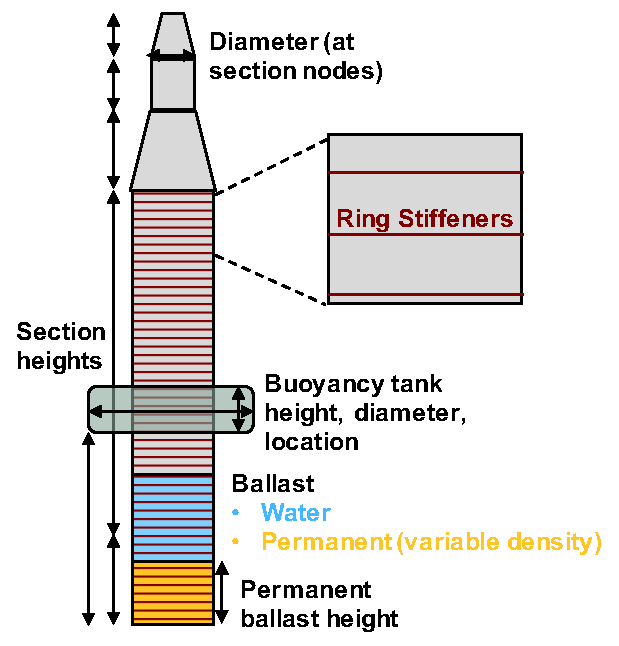
\includegraphics[width=2.2in]{figs/colGeom}
    \caption{Vertical column of frustums}
  \end{subfigure}
  \begin{subfigure}[b]{0.29\linewidth}
    \centering 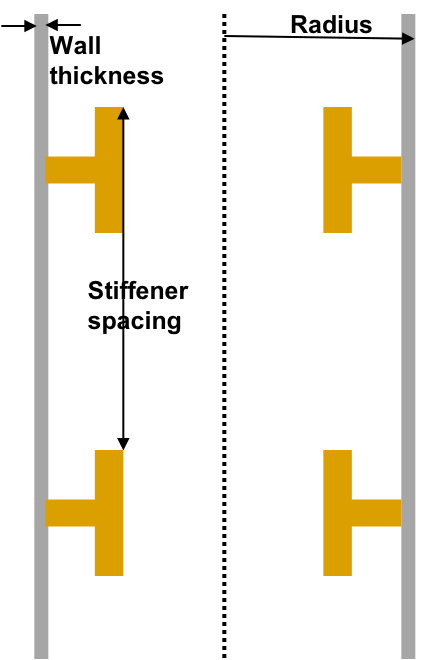
\includegraphics[width=1.8in]{figs/stiffenerCut}
    \caption{Vertical cross-section}
  \end{subfigure}
  \begin{subfigure}[b]{0.29\linewidth}
    \centering 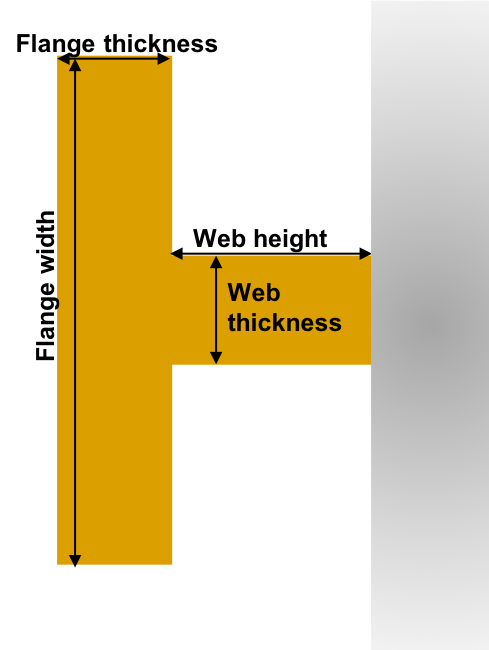
\includegraphics[width=1.8in]{figs/stiffenerZoom}
    \caption{Ring stiffener geometry}
  \end{subfigure}
  \caption{Vertical frustum geometry parameterization.}
  \label{fig:column}
\end{figure}

\subsubsection{Geometry}
To set the geometry of the base column from the \textit{FloatingSE} Group, use

{\footnotesize
  \begin{tabularx}{\linewidth}{ l l X }
    \textbf{Variable} & \textbf{Type} & \textbf{Description \& units} \\
    \texttt{base\_section\_height} & Float array ($nSection$) & Height of each section [$m$]\\
    \texttt{base\_outer\_diameter} & Float array ($nSection+1$) & Diameter at each section node (linear lofting between) [$m$] \\
    \texttt{base\_wall\_thickness} & Float array ($nSection+1$) & Wall thickness at each section node (linear lofting between) [$m$] \\
    \texttt{base\_freeboard} & Float scalar & Design height above waterline [$m$]\\
  \end{tabularx}
}

\subsubsection{Stiffeners}
The ring stiffener geometry is depicted in Figure \ref{fig:column}b--c and can be specified by,

{\footnotesize
  \begin{tabularx}{\linewidth}{ l l X }
    \textbf{Variable} & \textbf{Type} & \textbf{Description \& units} \\
    \texttt{base\_stiffener\_web\_height} & Float array ($nSection$) & Stiffener web height for each section [$m$]\\
    \texttt{base\_stiffener\_web\_thickness} & Float array ($nSection$) & Stiffener web thickness for each section [$m$]\\
    \texttt{base\_stiffener\_flange\_width} & Float array ($nSection$) & Stiffener flange width for each section [$m$]\\
    \texttt{base\_stiffener\_flange\_thickness} & Float array ($nSection$) & Stiffener flange thickness for each section [$m$]\\
    \texttt{base\_stiffener\_spacing} & Float array ($nSection$) & Stiffener spacing for each section [$m$]\\
  \end{tabularx}
}

\subsubsection{Auxiliary Columns}
To set the equivalent parameters for the set of
auxiliary-columns, merely substitute the word
``\texttt{auxiliary}'' for ``\texttt{base}'' in the above parameters.  Two
additional variables control the number and placement of the
auxiliary-columns,

{\footnotesize
  \begin{tabularx}{\linewidth}{ l l X }
    \textbf{Variable} & \textbf{Type} & \textbf{Description \& units} \\
    \texttt{number\_of\_auxiliary\_columns} & Integer scalar & Number of auxiliary columns in substructure (for spar set to 0)\\
    \texttt{radius\_to\_auxiliary\_column} & Float scalar & Centerline of base column to centerline of auxiliary column [$m$]\\
  \end{tabularx}
}

\subsubsection{Material Properties}
The material of the vertical columns is currently assumed to uniformly
be ASTM 992 steel.  Future developments will include the option to
select one of multiple material options for each section in each
cylinder.  Currently, to globally change to a different material, use
the variables,

{\footnotesize
  \begin{tabularx}{\linewidth}{ l l X }
    \textbf{Variable} & \textbf{Type} & \textbf{Description \& units} \\
    \texttt{material\_density} & Float scalar & Mass density (assumed steel) [$kg/m^3$]\\
    \texttt{E} & Float scalar & Young's modulus (of elasticity) [$N/m^2$]\\
    \texttt{G} & Float scalar & Shear modulus [$N/m^2$]\\
    \texttt{yield\_stress} & Float scalar & Elastic yield stress [$N/m^2$]\\
    \texttt{nu} & Float scalar & Poisson's ratio ($\nu$)\\
  \end{tabularx}
}

\subsubsection{Ballast}
Substructure columns with long drafts enhance dynamic stability by placing heavy
ballast at their keel (bottom point).  Bulkheads between column sections
help to keep the ballast in place, or serve as dividers between other
section roles.  The variables that govern the implementation of the
permanent ballast and bulkhead nodes are,

{\footnotesize
  \begin{tabularx}{\linewidth}{ l l X }
    \textbf{Variable} & \textbf{Type} & \textbf{Description \& units} \\
    \texttt{permanent\_ballast\_density} & Float scalar & Mass density of ballast material [$kg/m^3$]\\
    \texttt{base\_permanent\_ballast\_height} & Float scalar & Height above keel for permanent ballast [$m$]\\
    \texttt{base\_bulkhead\_nodes} & Boolean list ($nSection+1$) & Locations of internal bulkheads at section interfaces\\
  \end{tabularx}
}
As with the other geometry parameters, equivalent options exist with the
\texttt{auxiliary} prefix (instead of \texttt{base}), as well.

Variable ballast, as opposed to permanent ballast, is water that is
added or removed above the permanent ballast to achieve neutral buoyancy as the
operating conditions of the turbine change.  A discussion of variable
balance in the model is found in Section \ref{sec:static}.

\subsection{Pontoons and Support Structure}
Many substructure designs include the use of pontoons that form a truss
to connect the different components, usually columns, together.  In this
model, all of the pontoons are assumed to have the identical thin-walled
tube cross section and made of the same material as the rest of the
substructure.  The variables that govern pontoon cross section are,

{\footnotesize
  \begin{tabularx}{\linewidth}{ l l X }
    \textbf{Variable} & \textbf{Type} & \textbf{Description \& units} \\
    \texttt{pontoon\_outer\_diameter} & Float scalar & Diameter of all pontoon/truss elements [$m$]\\
    \texttt{pontoon\_wall\_thickness} & Float scalar & Thickness of all pontoon/truss elements [$m$]\\
  \end{tabularx}
}

\begin{figure}
  \begin{center}
    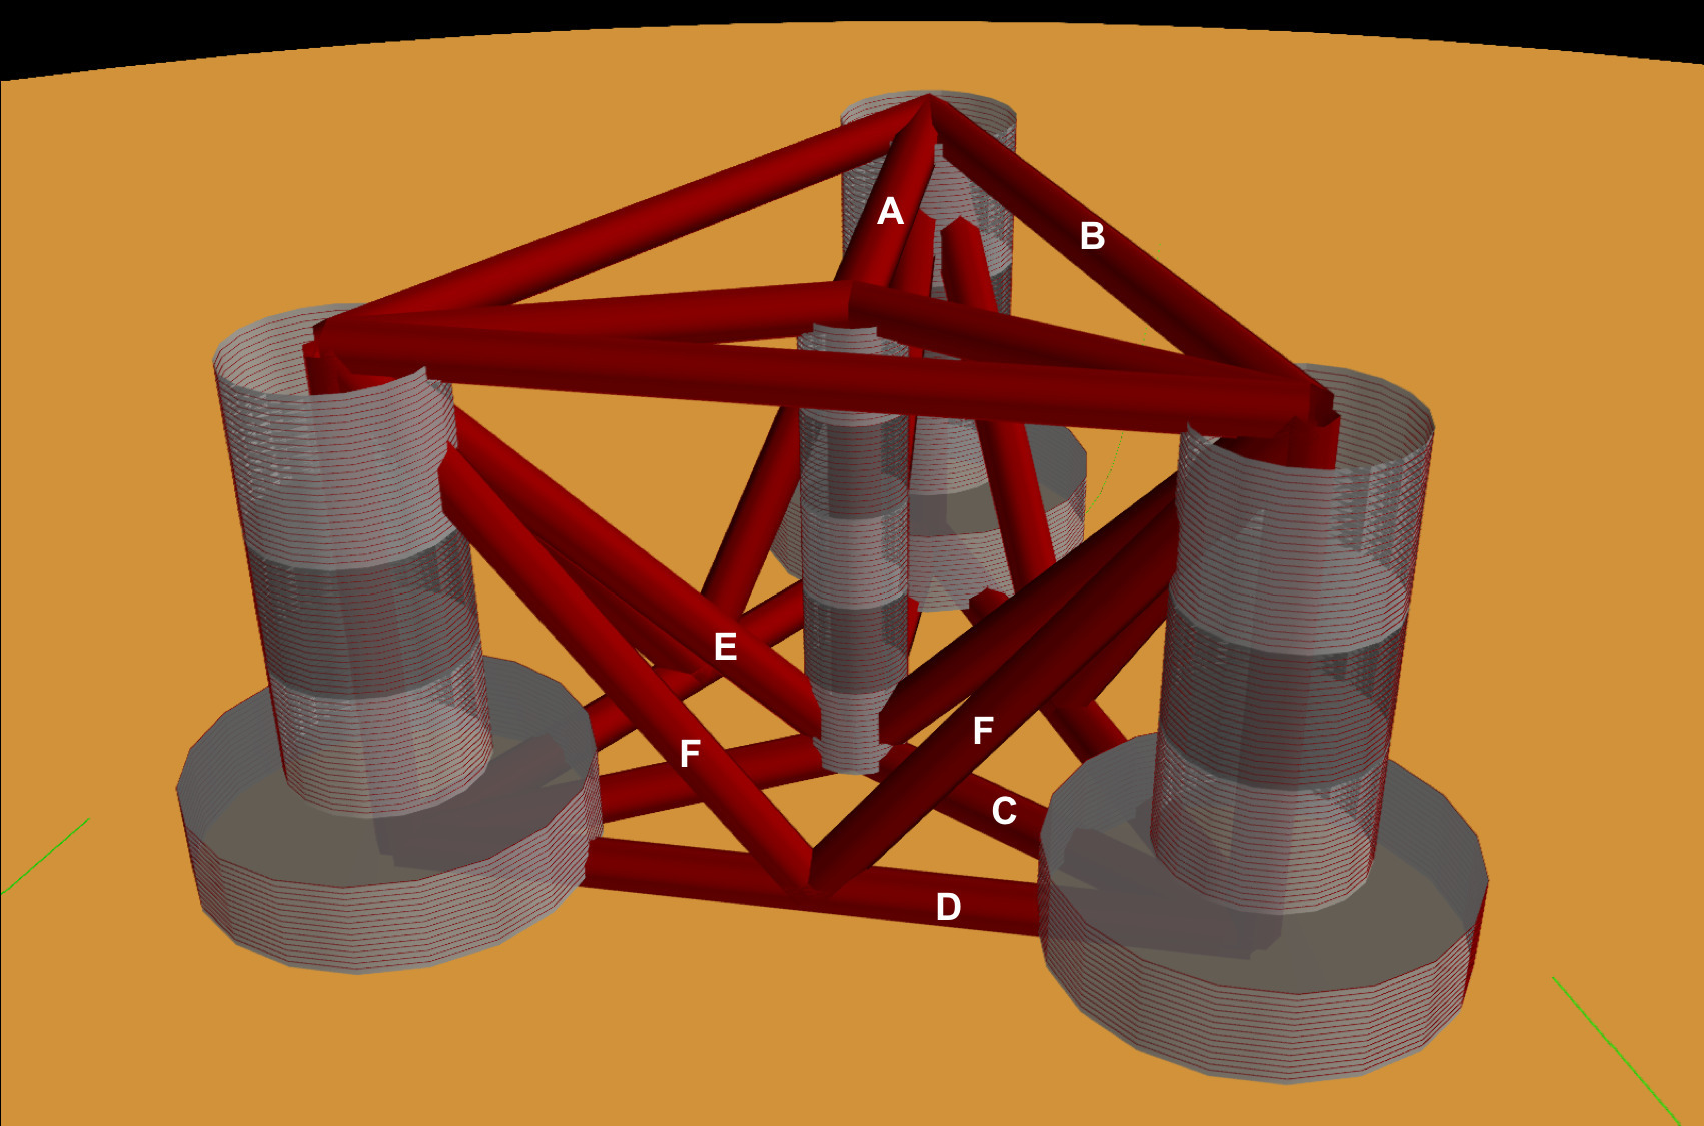
\includegraphics[width=4.5in]{figs/semi}
    \caption{Parameterization of truss elements in substructure.}
    \label{fig:pontoon}
  \end{center}
\end{figure}

The parameterization of the pontoon elements, the interconnecting truss
of the substructure, is based on the members shown in Figure
\ref{fig:pontoon}.  The members are broken out into the upper and lower
rings connecting the auxiliary columns, the upper and lower
base-to-auxiliary connections, the lower-base to upper-auxiliary cross
members, and the V-shaped cross members between auxiliary columns.  The
variables that drive this parameterization are,

{\footnotesize
  \begin{tabularx}{\linewidth}{ l l c X }
    \textbf{Variable} & \textbf{Type} & \textbf{Figure \ref{fig:pontoon}} & \textbf{Description \& units} \\
    \texttt{base\_pontoon\_attach\_lower} & Float scalar & & Lower z-coordinate on base where truss attaches [$m$]\\
    \texttt{base\_pontoon\_attach\_upper} & Float scalar & & Upper z-coordinate on base where truss attaches [$m$]\\
    \texttt{upper\_attachment\_pontoons} & Boolean & A & Upper base-to-auxiliary connecting pontoons\\
    \texttt{lower\_attachment\_pontoons} & Boolean & C & Lower base-to-auxiliary connecting pontoons\\
    \texttt{cross\_attachment\_pontoons} & Boolean & E & Lower-Upper base-to-auxiliary connecting cross braces\\
    \texttt{upper\_ring\_pontoons} & Boolean & B & Upper ring of pontoons connecting auxiliary columns\\
    \texttt{lower\_ring\_pontoons} & Boolean & D & Lower ring of pontoons connecting auxiliary columns\\
    \texttt{outer\_cross\_pontoons} & Boolean & F & Auxiliary ring connecting V-cross braces\\
  \end{tabularx}
}


\subsection{Mooring Lines}
The mooring system is described by the number of lines, their geometry,
and their interface to the substructure.  The mooring diameter is
specified directly and determines the breaking load and stiffness of the
chain.  The mooring lines attach to the substructure at the ``fairlead''
distance below the water plane, as shown in Figure \ref{fig:diagram}.
The lines can attach directly to a substructure column or at a some
offset from the outer surface.  Note that bridle connections are not yet
implemented, but could be done some quickly if there was sufficient
need.  The mooring lines attach to the sea floor at a variable distance
from the substructure centerline and their total length is governed by
their scope ratio, a ratio of the line length to the distance from the
fairlead connection to the sea floor,
\[
  L = ScopeRatio \times \left( z_{fairlead} - z_{seafloor} \right)
\]
The variables that control the mooring system geometry are the following,

{\footnotesize
  \begin{tabularx}{\linewidth}{ l l X }
    \textbf{Variable} & \textbf{Type} & \textbf{Description \& units} \\
    \texttt{number\_of\_mooring\_lines} & Integer scalar & Number of mooring lines evenly spaced around structure\\
    \texttt{mooring\_diameter} & Float scalar & Diameter of mooring line/chain [$m$]\\
    \texttt{fairlead} & Float scalar & Distance below waterline for attachment [$m$]\\
    \texttt{fairlead\_offset\_from\_shell} & Float scalar & Offset from shell surface for mooring attachment [$m$] \\
    \texttt{scope\_ratio} & Float scalar & Ratio of line length to distance to sea floor (from fairlead)\\
    \texttt{anchor\_radius} & Float scalar & Distance from centerline to sea floor landing [$m$]\\
    \texttt{drag\_embedment\_extra\_length} & Float scalar & Extra length beyond sea flor landing to ensure anchors only see horizontal forces [$m$]\\
  \end{tabularx}
}

By default, the mooring system is assumed to use a steel chain with drag
embedment anchors. As a placeholder, other mooring and anchor types are available for
selection, but their behavior has not yet been tested or verified.
Alternative mooring line types include nylon, polyester, steel wire rope
(IWRC) and fiber-core wire rope.  The only alternative anchor type is
currently suction pile anchors, but there are plans to include gravity
anchors as well.  These alternatives can be accessed through the
parameters,

{\footnotesize
  \begin{tabularx}{\linewidth}{ l l X }
    \textbf{Variable} & \textbf{Type} & \textbf{Description \& units} \\
    \texttt{mooring\_type} & Enumerated & Options are CHAIN, NYLON, POLYESTER, FIBER, or IWRC\\
    \texttt{anchor\_type} & Enumerated & Options are SUCTIONPILE or DRAGEMBEDMENT\\
  \end{tabularx}
}


\subsection{Mass and Cost Scaling}
The mass of all components in the modeled substructure is captured
through calculation of each components' volume and multiplying by its material
density.  This applies to the frustum shells, the ring stiffeners, the
permanent and water ballast, the pontoons, and the mooring lines.
However, the model also acknowledges that the modeled substructure is
merely an approximation of an actual substructure and various secondary
elements are not captured.  These include ladders, walkways, handles,
finishing, paint, wiring, etc.  To account for these features en masse,
multipliers of component masses are offered as parameters for the user,

{\footnotesize
  \begin{tabularx}{\linewidth}{ l l X }
    \textbf{Variable} & \textbf{Type} & \textbf{Description \& units} \\
    \texttt{bulkhead\_mass\_factor}     & Float scalar     & Scaling for unaccounted bulkhead mass\\
    \texttt{ring\_mass\_factor}         & Float scalar     & Scaling for unaccounted stiffener mass\\
    \texttt{shell\_mass\_factor}        & Float scalar     & Scaling for unaccounted shell mass\\
    \texttt{column\_mass\_factor}       & Float scalar    & Scaling for unaccounted column mass\\
    \texttt{outfitting\_mass\_fraction} & Float scalar    & Fraction of additional outfitting mass for each column\\
  \end{tabularx}
}

The costs of the substructure components are set by constant multipliers
of their mass.  These multiplier are difficult to determine empirically
due to the proprietary nature of cost data.  The values for the
variables below are simply casual rules-of-thumb within NREL.

{\footnotesize
  \begin{tabularx}{\linewidth}{ l l X }
    \textbf{Variable} & \textbf{Type} & \textbf{Description \& units} \\
    \texttt{ballast\_cost\_rate}        & Float scalar   & Cost factor for ballast mass [$USD/kg$]\\
    \texttt{tapered\_col\_cost\_rate}    & Float scalar  & Cost factor for column mass [$USD/kg$]\\
    \texttt{outfitting\_cost\_rate}     & Float scalar  & Cost factor for outfitting mass [$USD/kg$]\\
    \texttt{mooring\_cost\_rate}        & Float scalar     & Cost factor for mooring mass [$USD/kg$]\\
    \texttt{pontoon\_cost\_rate}        & Float scalar   & Cost factor for pontoons [$USD/kg$]\\
  \end{tabularx}
}
